\documentclass[
]{jss}

\usepackage[utf8]{inputenc}

\providecommand{\tightlist}{%
  \setlength{\itemsep}{0pt}\setlength{\parskip}{0pt}}

\author{
Namgil Lee\\Kangwon National University \And Heon-Young Yang\\Kangwon National University \And Sung-Ho Kim\\KAIST
}
\title{\pkg{VARshrink}: Shrinkage Estimation Methods for Vector Autoregressive
Models}

\Plainauthor{Namgil Lee, Heon-Young Yang, Sung-Ho Kim}
\Plaintitle{VARshrink: Shrinkage Estimation Methods for Vector Autoregressive Models}
\Shorttitle{\pkg{VARshrink}}

\Abstract{
We introduce an \proglang{R} software package, \pkg{VARshrink}, for
providing shrinkage estimation methods for vector autoregressive (VAR)
models. Contrary to the standard ordinary least squares method,
shrinkage estimation methods can be applied to high-dimensional VAR
models with dimensionality greater than the number of observations.
While existing \proglang{R} packages for VAR shrinkage are mostly based
on parametric, Bayesian estimation methods using informative priors, the
\pkg{VARshrink} aims to be an integrative \proglang{R} package
delivering nonparametric, parametric, and semiparametric methods in a
unified and consistent manner. The current version of \pkg{VARshrink}
contains four shrinkage estimation methods, which are the multivarate
ridge regression, a nonparametric shrinkage method, a full Bayesian
approach using noninformative priors, and a semiparametric Bayesian
approach using informative priors. VAR estimation problems are
formulated as a multivariate regression form, so that all the shrinkage
estimation methods can be run by one interface function named
\code{VARshrink()}. We clearly present mathematical expressions of
shrinkage estimators of the shrinkage estimation methods. The effective
number of parameters can be calculated based on a shrinkage intensity
parameter value, which plays an important role for further statistical
analyses. We provide a sample \proglang{R} code for demonstration of the
package and comparison of performances of the shrinkage estimation
methods.
}

\Keywords{Bayes estimation, vector autoregression (VAR), high-dimensionality, shrinkage, multivariate time series}
\Plainkeywords{Bayes estimation, vector autoregression (VAR), high-dimensionality, shrinkage, multivariate time series}

%% publication information
%% \Volume{50}
%% \Issue{9}
%% \Month{June}
%% \Year{2012}
%% \Submitdate{}
%% \Acceptdate{2012-06-04}

\Address{
    Namgil Lee\\
  Kangwon National University\\
  Department of Information Statistics, Kangwon National University,
  Chuncheon, Gangwon 24341, South Korea\\
  E-mail: \email{namgil.lee@kangwon.ac.kr}\\
  URL: \url{https://sites.google.com/site/namgil}\\~\\
        Sung-Ho Kim\\
  KAIST\\
  Department of Mathematical Sciences, KAIST, Daejeon 305-701, South Korea\\
  E-mail: \email{sung-ho.kim@kaist.edu}\\
  
  }

% Pandoc header

\usepackage{amsmath} \usepackage{amsfonts} \usepackage{array}

\begin{document}

\hypertarget{introduction}{%
\section{Introduction}\label{introduction}}

\label{sec:intro}

Let \(\mathbf{y}_t = (y_{t1},y_{t2},\ldots,y_{tK})^\top\) denote a
\(K\times 1\) vector of endogenous variables. A vector autoregressive
(VAR) model of order \(p\) can be expressed as
\begin{equation}    \label{VAReqnA}
    \mathbf{y}_t = \mathbf{A}_1 \mathbf{y}_{t-1} + \cdots + \mathbf{A}_p \mathbf{y}_{t-p} + \mathbf{C} \mathbf{d}_t + \boldsymbol\epsilon_t,
    \end{equation} where \(\mathbf{d}_t\) is an \(L\times 1\) vector of
deterministic regressors, \(\boldsymbol\epsilon_t\) is a \(K\times 1\)
noise vector, and \(\mathbf{A}_1,\ldots,\mathbf{A}_p\) and
\(\mathbf{C}\) are coefficient matrices \citep{Hamilton94, Tsay05}.

\hypertarget{backgrounds}{%
\subsection{Backgrounds}\label{backgrounds}}

Recently, several \proglang{R} packages have been developed for
parameter estimation and forecasting using stochastic time series
models. The \pkg{forecast} package provides various methods and tools
for univariate time series models such as the ARIMA and ETS models
\citep{Hyndman18}. The \pkg{MTS} package has been developed for a wide
variety of multivariate linear time series models and multivariate
volatility models such as the VARMA, multivariate EWMA, and
low-dimensional BEKK models \citep{Tsay18}. The \pkg{vars} package
provides methods for multivariate time series analysis using the VAR,
SVAR, and SVEC models \citep{Pfaff18}.

In this study, we focus on shrinkage estimation of VAR model parameters.
Shrinkage estimation methods have been playing crucial roles in
high-dimensional statistical modeling; see, e.g.,
\citet{Beltra2013shrinkageEEG}, \citet{Bohm2009shrinkage},
\citet{Fiecas2011aoas} and \citet{LedoitWolf2004shrinkcov}. For VAR
models, several shrinkage estimation methods have been suggested such as
a Stein-type nonparametric shrinkage estimation method \citep{Rhein07c},
Bayesian VARs using informative priors
\citep{Banbura10, Doan84, Koop10BayesianVAR, Litterman86}, Bayesian VARs
using noninformative priors \citep{Ni05, Sun04}, and a semiparametric
Bayesian approach adopting a modified \(K\)-fold cross validation
\citep{LeeChoiKim2016}.

Due to its popularity in macroeconomic time series analysis, several
Bayesian VAR methods have been implemented in \proglang{R} packages. For
example, the function \code{BVAR()} in \pkg{MTS} implements a Bayesian
VAR method using an informative prior \citep{Tsay18}; the package
\pkg{bvarsv} implements Bayesian VAR models with stochastic volatility
and time-varying parameters
\citep{Krueger2015bvarsv, Koop10BayesianVAR, Primiceri2005timevarying}.

On the other hand, we note that other types of shrinkage methods which
have been implemented for other purposes than multivariate time series
analysis can be applied to shrinkage estimation of VAR parameters. For
instance, the function \code{cov.shrink()} in the package \pkg{corpcor}
has been implemented to compute shrinkage estimates of covariances, but
it has been applied to estimate VAR coefficients in
\citeauthor{Rhein07c}
\citetext{\citeyear{Rhein07c}; \citealp{Schafer17}}. Moreover, we note
that VAR models can be reformulated into multivariate regression
problems, so that penalized least squares methods can be used for
shrinkage estimation of VAR parameters, e.g., the functions
\code{lm.gls()} for generalized least squares and \code{lm.ridge()} for
ridge regression in the package \pkg{MASS} \citep{Ripley18}; the
function \code{glmnet()} for Lasso and Elastic-Net regularized
generalized linear models in the package \code{glmnet()}
\citep{Frideman18}; the function \code{linearRidge()} for ridge
regression in the package \pkg{ridge} \citep{Moritz18}.

\hypertarget{main-purpose}{%
\subsection{Main Purpose}\label{main-purpose}}

While Bayesian approaches have been widely used in the literature, we
note that nonparametric and semiparametric approaches have advantages in
the case of high-dimensional VARs with more than several hundreds of
time series variables due to their relatively low computational costs
\citep{Rhein07c}. Despite of their relatively high computational costs,
Bayesian approaches can impose proper assumptions on the multivariate
time series data flexibly, such as VAR roots near unity and correlations
between noise processes \citep{LeeChoiKim2016}. In this sense, a
semiparametric approach can be a trade-off between nonparametric and
parametric approaches \citep{LeeChoiKim2016}.

In this study, we developed an integrative \proglang{R} package,
\pkg{VARshrink}, for implementing nonparametric, parametric, and
semiparametric approaches for shrinkage estimation of VAR model
parameters. By providing a simple interface function,
\code{VARshrink()}, for running various types of shrinkage estimation
methods, the performance of the methods can be easily compared. We note
that the package \pkg{vars} implemented an ordinary least squares method
for VAR models by the function \code{VAR()}. The function
\code{VARshrink()} was built to extend \code{VAR()} to shrinkage
estimation methods, so that the \pkg{VARshrink} package takes advantage
of the tools and methods available in the \pkg{vars} package. For
example, we demonstrate the use of model selection criteria such as AIC
and BIC in this paper, where the methods \code{AIC(), BIC(),} and
\code{logLik()} can handle multivariate t-distribution and the effective
number of parameters in \pkg{VARshrink}.

This paper is organized as follows. In Section 2, we explain the general
distribution assumption for the noise term in a Bayesian framework. We
also present the formulation of VAR models in a multivariate regression
problem, which simplifies implementation of the package. In Section 3,
we describe the common interface function and the four shrinkage
estimation methods included in the package. We clearly present closed
form expressions for the shrinkage estimators inferred by the shrinkage
methods, so that we can indicate the role of the shrinkage intensity
parameters in each method. In addition, we explain how the effective
number of parameters can be computed for shrinkage estimators. In
Section 4, we present numerical experiments using benchmark data and
simulated data for comparing performances of the shrinkage estimation
methods. Discussion and conclusions are provided in Section 5.

\begin{center}\rule{0.5\linewidth}{\linethickness}\end{center}

\hypertarget{models}{%
\section{Models}\label{models}}

In the VAR model in \eqref{VAReqnA}, we assume that the noise vectors
are independent and identically distributed from a scale mixture of
multivariate normal distributions, including multivariate normal
distributions, multivariate t-distributions \citep{Ni05}, and
multivariate Laplace distributions (MLD) \citep{Eltoft06}. By
incorporating scale mixture distributions in the model assumption, we
can handle outliers appropriately and produce robust estimates
\citep{West84}. In specific, we consider that a noise vector can be
expressed as a product \begin{equation}
    \label{productZD}
    \boldsymbol\epsilon_t = \mathbf{z}_t q_t^{-1/2},
    \end{equation} where
\(\mathbf{z}_t \sim \text{N}_K(\mathbf{0}, \mathbf{\Sigma})\) is a
\(K\times 1\) vector having a multivariate normal distribution with the
mean vector of zeros and the covariance matrix of \(\boldsymbol\Sigma\),
and \(q_t \sim \text{Gamma}(\nu/2, \nu/2)\) is a random variable having
a gamma distribution with shape \(\alpha = \nu/2\) and rate
\(\beta = \nu/2\). The following statements describe characteristics of
the distributions in more detail.

\begin{itemize}
\item
  If \(1<\nu<\infty\), then \(\boldsymbol\epsilon_t\) has a multivariate
  t-distribution with the degree of freedom \(\nu\). The probability
  density function (p.d.f.) for \(\boldsymbol\epsilon_t\) can be
  expressed as \begin{equation}
        \label{pdf_multiv_t}
        f\left( \boldsymbol\epsilon_t \right) = g\left( \left\| \mathbf{V}^{-1/2} \boldsymbol\epsilon_t \right\|^2 \right) \left| \mathbf{V} \right|^{-1/2},
        \end{equation} with \begin{equation}
        g(x) \propto \left(1 + \frac{x}{\nu} \right)^{-(\nu+K)/2}.
        \end{equation} Define \begin{equation}
        \label{hfunction}
        h(x) = -2 \frac{\text{d}}{\text{d}x}  \log g(x) = \frac{\nu + K}{\nu + x}.
        \end{equation}
\item
  If \(\nu \rightarrow \infty\), the distribution for
  \(\boldsymbol\epsilon_t\) converges to the multivariate normal
  distribution, \(\text{N}_K(\mathbf{0}, \mathbf{\Sigma})\). The p.d.f.
  for \(\boldsymbol\epsilon_t\) can be expressed as \eqref{pdf_multiv_t}
  with \(g(x) \propto \exp(-x/2)\) and \(h(x) = 1\).
\item
  If \(\nu = 1\), the distribution for \(\boldsymbol\epsilon_t\)
  converges to the multivariate Cauchy distribution. The p.d.f. for
  \(\boldsymbol\epsilon_t\) can be expressed as \eqref{pdf_multiv_t}
  with \(g(x) \propto (1+x)^{-(1+K)/2}\) and \(h(x) = (1+K)/(1+x)\).
\item
  If \(\nu \approx 0\), the distribution cannot be obtained in a simple
  closed form, but the p.d.f. for \(\boldsymbol\epsilon_t\) can still be
  written with \(g(x) \propto x^{-K/2}\) and \(h(x) = K/x\).

  In this case, the expression for \(q_t\) during the iteration process
  in semiparametric Bayesian approach \citep{LeeChoiKim2016} is
  equivalent to the IRLS procedure for L1 norm minimization
  \citep{Chartrand08}; see Section 3.4 for more detail.

  In addition, we note that the p.d.f.
  \(f^{MLD} (\boldsymbol\epsilon_t)\) of the multivariate Laplace
  distribution (MLD) can be expressed as in \eqref{pdf_multiv_t} with \[
        g^{MLD}(x) \propto \frac{ \tilde{K}_{(K-2)/2} (\sqrt{2x/\beta}) }{ (\sqrt{ \beta x/2 })^{(K-2)/2} }
        \] for some \(\beta>0\) \citep{Eltoft06}. Since
  \(\tilde{K}_\alpha (z)\), the modified Bessel function of the second
  kind, can be approximated by
  \(\tilde{K}_\alpha (z) \approx \Gamma(\alpha) 2^{\alpha-1} z^{-\alpha}\)
  for small values of \(0<z\leq \sqrt{\alpha+1}\), the p.d.f. of MLD can
  be approximated by \(g^{MLD} (x) \propto x^{-K/2+1}\) for small values
  of \(0<x\leq \sqrt{K\beta/4}\). Therefore, we consider that the
  multivariate t-distribution is approximately close to the MLD when
  \(\nu\rightarrow 0\).
\end{itemize}

In general, we can rewrite the model equation \eqref{VAReqnA} in the
form of a multivariate regression as
\begin{equation}    \label{VAReqnPsi}
    \mathbf{y}_t    =   \mathbf{\Psi}^\top \mathbf{x}_t + \boldsymbol{\epsilon}_t,
    \end{equation} where
\(\mathbf{\Psi} = (\mathbf{A}_1, \mathbf{A}_2, \ldots, \mathbf{A}_p, \mathbf{C})^\top\)
is a \((Kp + L) \times K\) matrix of coefficients,
\(\mathbf{x}_t = (\mathbf{y}_{t-1}^\top, \ldots, \mathbf{y}_{t-p}^\top, \mathbf{d}_t^\top)^\top\)
is a \((Kp + L)\times 1\) vector of regressors. For estimation of VAR
parameters from the observed time series data
\(\mathbf{y}_1, \mathbf{y}_2, \ldots, \mathbf{y}_T\), we define data
matrices as \begin{equation}
    \begin{split}
    \mathbf{Y} &= ( \mathbf{y}_{p+1}, \mathbf{y}_{p+2}, \ldots, \mathbf{y}_{T} )^\top \in \mathbb{R}^{N \times K},
    \\
    \mathbf{X} &= ( \mathbf{x}_{p+1}, \mathbf{x}_{p+2}, \ldots, \mathbf{x}_{T} )^\top \in \mathbb{R}^{N \times (Kp + L)},
    \end{split}
    \end{equation} with \(N = T-p\). Then, we can rewrite
\eqref{VAReqnPsi} in a matrix form as \begin{equation}
    \label{VAReqnMat}
    \mathbf{Y} = \mathbf{X} \mathbf{\Psi} + \mathbf{E} \in \mathbb{R}^{N \times K},
    \end{equation} with
\(\mathbf{E} = (\boldsymbol\epsilon_{p+1}, \ldots, \boldsymbol\epsilon_T)^\top\)
and \(N = T-p\).

\begin{center}\rule{0.5\linewidth}{\linethickness}\end{center}

\hypertarget{sec:methods}{%
\section{Shrinkage Estimation Methods}\label{sec:methods}}

In this section, we will describe the shrinkage estimation methods
implemented in this package. The methods are used for estimating the VAR
coefficient matrix \(\mathbf{\Psi}\) alone or both of the
\(\mathbf{\Psi}\) and \(\mathbf{\Sigma}\) in \eqref{VAReqnMat}.

We provide a common \proglang{R} function interface \code{VARshrink()}
for running the estimation methods, which is defined by

\begin{verbatim}
VARshrink(y, p = 1, type = c("const", "trend", "both", "none"),
  season = NULL, exogen = NULL, method = c("ridge", "ns", "fbayes",
  "sbayes", "kcv"), lambda = NULL, lambda_var = NULL, dof = Inf, ...)
\end{verbatim}

The input arguments are described as follows.

\begin{itemize}
\tightlist
\item
  \code{y}: A T-by-K matrix of endogenous variables
\item
  \code{p}: Integer for the lag order
\item
  \code{type}: Type of deterministic regressors to include.

  \begin{enumerate}
  \def\labelenumi{\arabic{enumi})}
  \tightlist
  \item
    ``const'' - the constant: \(\mathbf{d}_t = 1\).
  \item
    ``trend'' - the trend: \(\mathbf{d}_t = t\).
  \item
    ``both'' - both the constant and the trend:
    \(\mathbf{d}_t = (t, 1)^\top\).
  \item
    ``none'' - no deterministic regressors.
  \end{enumerate}
\item
  \code{season}: An integer value of frequency for inclusion of centered
  seasonal dummy variables.
\item
  \code{exogen}: A T-by-L matrix of exogenous variables.
\item
  \code{method}:

  \begin{enumerate}
  \def\labelenumi{\arabic{enumi})}
  \tightlist
  \item
    ``ridge'' - multivariate ridge regression.
  \item
    ``ns'' - a Stein-type nonparametric shrinkage method.
  \item
    ``fbayes'' - a full Bayesian shrinkage method using noninformative
    priors.
  \item
    ``sbayes'' - a semiparametric Bayesian shrinkage method using
    parameterized cross validation.
  \item
    ``kcv'' - a semiparametric Bayesian shrinkage method using K-fold
    cross validation
  \end{enumerate}
\item
  \code{lambda, lambda_var}: Shrinkage parameter value(s). Use of this
  parameter is slightly different for each method: the same value does
  not imply the same shrinkage estimates. See description in the
  following subsections for the use of shrinkage parameters in each
  method.
\item
  \code{dof}: Degree of freedom of multivariate t-distribution for
  noise. Valid only for \code{method = "fbayes"} and
  \code{method = "sbayes"}. \code{dof = Inf} means multivariate normal
  distribution.
\end{itemize}

The output value is an object of class ``varshrinkest'', which inherits
the class ``varest'' in the package \pkg{vars}, and an object of class
``varest'' can be obtained by the function \code{VAR()} in the package
\pkg{vars}. The input arguments and the output value indicate that
\code{VARshrink()} is an extension of \code{VAR()} in the \pkg{vars}
package. As a result, almost all the methods and functions included in
the package \pkg{vars} are available for the package \pkg{VARshrink},
such as \code{fevd(), Phi(), plot()}. The methods and functions
available in the \pkg{VARshrink} package are summarized in Table
\ref{tab:methods}. The names of the functions for class ``varshrinkest''
has suffix "\_sh" in order to distinguish them from the functions for
class ``varest''. We remark that the classes ``varshrinkest'',
``varshirf'', and ``varshsum'' inherit the classes ``varest'',
``varirf'', and ``varsum'' of the \pkg{vars} package, respectively.

\begin{CodeChunk}
\begin{table}[t]

\caption{\label{tab:unnamed-chunk-1}\label{tab:methods}Structure of the package VARshrink.}
\centering
\begin{tabular}{>{\raggedright\arraybackslash}p{7em}|>{\raggedright\arraybackslash}p{7em}|>{\raggedright\arraybackslash}p{7em}|>{\raggedright\arraybackslash}p{7em}}
\hline
Function or method & Class & Methods for class & Functions for class\\
\hline
VAR & varshrinkest, varest & coef, fevd, fitted, irf, logLik, Phi, plot, predict, print, Psi, resid, summary & Acoef\_sh, arch.test\_sh, Bcoef\_sh, BQ\_sh, causality\_sh, normality.test\_sh, restrict\_sh, roots\_sh, serial.test\_sh, stability\_sh\\
\hline
fevd & varfevd & plot, print & \\
\hline
irf & varshirf, varirf & plot, print & \\
\hline
predict & varprd & plot, print & fanchart\\
\hline
summary & varshsum, varsum & print & \\
\hline
arch.test\_sh & varcheck & plot, print & \\
\hline
normality.test\_sh & varcheck & plot, print & \\
\hline
serial.test\_sh & varcheck & plot, print & \\
\hline
stability\_sh & varstabil & plot, print & \\
\hline
\end{tabular}
\end{table}

\end{CodeChunk}

\hypertarget{multivariate-ridge-regression}{%
\subsection{Multivariate Ridge
Regression}\label{multivariate-ridge-regression}}

The ridge regression method is a kind of penalized least squares (PLS)
method, which produces a biased estimate of the VAR coefficient
\citep{Hoerl70}. Formally speaking, the ridge regression estimator of
\(\mathbf{\Psi}\) can be obtained by minimizing the penalized sum of
squared prediction errors (SSPE) as \begin{equation}
    \widehat{ \mathbf{\Psi} }^{\text{R}} (\lambda) =
    \arg\min_{\mathbf{\Psi}}
    \
    \frac{1}{N}
    \left\|\mathbf{Y}  -  \mathbf{X} \mathbf{\Psi} \right\|_F^2  +
    \lambda \left\| \mathbf{\Psi} \right\|_F^2,
    \end{equation} where
\(\|\mathbf{A}\|_F = \sqrt{ \sum_{i} \sum_{j} a_{ij}^2 }\) is the
Frobenius norm of a matrix \(\mathbf{A}\), \(N = T-p\), and
\(\lambda \geq 0\) is called the regularization parameter or the
shrinkage parameter. The ridge regression estimator
\(\widehat{ \mathbf{\Psi} }^\text{R} (\lambda)\) can be expressed in the
closed form \begin{equation}
    \widehat{ \mathbf{\Psi} }^\text{R} (\lambda) =
    \left( \mathbf{X}^\top \mathbf{X} + N \lambda \mathbf{I} \right)^{-1} \mathbf{X}^\top \mathbf{Y},
    \qquad
    \lambda \geq 0.
    \end{equation}

The shrinkage parameter \(\lambda\) for the ridge regression can be
automatically determined by using the generalized cross-validation (GCV)
\citep{Golub79}. The GCV selects the value of \(\lambda\) where the GCV
score given below is minimized: \begin{equation}
    GCV(\lambda) = \frac{1}{N} \left\| (\mathbf{I} - \mathbf{H}(\lambda) \mathbf{Y} )  \right\|^2_\text{F}
    \left/
    \left[ \frac{1}{N} Trace(\mathbf{I} - \mathbf{H}(\lambda) ) \right]^2
    \right. ,
    \end{equation} where
\(\mathbf{H}(\lambda) = \mathbf{X}^\top \left(\mathbf{X}^\top \mathbf{X} + N \lambda \mathbf{I} \right)^{-1} \mathbf{X}^\top\).

In this package, the interface to the shrinkage estimation methods is
provided by the function \code{VARshrink(method = "ridge", \ldots)}. If
the input argument \code{lambda} is set at a value or a vector of
values, then corresponding GCV score is computed automatically for each
\(\lambda\) value, and the VAR coefficients with the smallest GCV score
is selected. If \code{lambda = NULL}, then the default value of
\code{c(0.0001, 0.0005, 0.001, 0.005, ..., 10, 50)} is used.

For example, simulated time series data of length \(T=100\) were
generated based on a multivariate normal distribution for noise and a
VAR model with \(p=1\), \(K=2\), \(\mathbf{A}_1 = 0.5\mathbf{I}_2\),
\(\mathbf{C}=(0.2, 0.7)^\top\), and
\(\mathbf{\Sigma} = 0.1^2\mathbf{I}_2\) as follows:

\begin{CodeChunk}

\begin{CodeInput}
R> set.seed(1000)
R> myCoef <- list(A = list(matrix(c(0.5, 0, 0, 0.5), 2, 2)), c = c(0.2, 0.7))
R> myModel <- list(Coef = myCoef, Sigma = diag(0.1^2, 2), dof = Inf)
R> Y <- simVARmodel(numT = 100, model = myModel, burnin = 10)
R> resu_estim <- list()
\end{CodeInput}
\end{CodeChunk}

Then, the multivariate ridge regression can be carried out for VAR
models as follows. The result printed on the screen shows all the
\code{lambda} values considered and the corresponding GCV values. The
VAR parameters are estimated using the lambda value with the minimum GCV
value.

\begin{CodeChunk}

\begin{CodeInput}
R> resu_estim$`Ridge regression` <-
R+   VARshrink(Y, p = 1, type = "const", method = "ridge", lambda = NULL)
R> resu_estim$`Ridge regression`
\end{CodeInput}

\begin{CodeOutput}

VAR Shrinkage Estimation Results:
================================= 

Estimated coefficients for equation y1: 
======================================= 
Call:
y1 = y1.l1 + y2.l1 + const 

     y1.l1      y2.l1      const 
0.61424699 0.07318362 0.05264740 


Estimated coefficients for equation y2: 
======================================= 
Call:
y2 = y1.l1 + y2.l1 + const 

    y1.l1     y2.l1     const 
0.1195550 0.3254618 0.9055450 


lambda: 1e-04 5e-04 0.001 0.005 0.01 0.05 0.1 0.5 1 5 10 50 (estimated: TRUE) 
GCV:  0.0187 0.0186 0.0186 0.0192 0.02 0.0227 0.025 0.0647 0.1506 0.8406 1.2754 1.9329 
\end{CodeOutput}
\end{CodeChunk}

The method \code{summary()} is available for objects of class
``varshrinkest'' as follows:

\begin{CodeChunk}

\begin{CodeInput}
R> summary(resu_estim$`Ridge regression`)
\end{CodeInput}

\begin{CodeOutput}

VAR Shrinkage Estimation Results:
=================================== 
Endogenous variables: y1, y2 
Deterministic variables: const 
Sample size: 99 
Log Likelihood: 188.793 
Roots of the characteristic polynomial:
0.6419 0.2978
Call:
VARshrink(y = Y, p = 1, type = "const", method = "ridge", lambda = NULL)


Estimation results for equation y1: 
=================================== 
y1 = y1.l1 + y2.l1 + const 

      Estimate Std. Error t value Pr(>|t|)    
y1.l1  0.61425    0.07636   8.045 2.27e-12 ***
y2.l1  0.07318    0.07549   0.969    0.335    
const  0.05265    0.10888   0.484    0.630    
---
Signif. codes:  0 '***' 0.001 '**' 0.01 '*' 0.05 '.' 0.1 ' ' 1


Residual standard error: 0.08913 on 96.16244 degrees of freedom
Multiple R-Squared: 0.3864, Adjusted R-squared: 0.3747 
F-statistic: 32.95 on 1.837559 and 96.16244 DF,  p-value: 4.725e-11 


Estimation results for equation y2: 
=================================== 
y2 = y1.l1 + y2.l1 + const 

      Estimate Std. Error t value Pr(>|t|)    
y1.l1  0.11955    0.08632   1.385 0.169249    
y2.l1  0.32546    0.08534   3.814 0.000242 ***
const  0.90555    0.12308   7.357  6.3e-11 ***
---
Signif. codes:  0 '***' 0.001 '**' 0.01 '*' 0.05 '.' 0.1 ' ' 1


Residual standard error: 0.1008 on 96.16244 degrees of freedom
Multiple R-Squared: 0.1219, Adjusted R-squared: 0.1051 
F-statistic: 7.263 on 1.837559 and 96.16244 DF,  p-value: 0.00157 



Scale matrix, Sigma, of multivariate t distribution for noise:
           y1         y2
y1  0.0077160 -0.0006829
y2 -0.0006829  0.0098611

Degrees of freedom of multivariate t distribution for noise:
[1] Inf

Correlation matrix of Sigma:
         y1       y2
y1  1.00000 -0.07829
y2 -0.07829  1.00000
\end{CodeOutput}
\end{CodeChunk}

\hypertarget{nonparametric-shrinkage-ns}{%
\subsection{Nonparametric Shrinkage
(NS)}\label{nonparametric-shrinkage-ns}}

The nonparametric shrinkage (NS) estimation method for VAR models,
proposed by \citet{Rhein07c}, produces an estimate of \(\mathbf{\Psi}\)
based on a James-Stein type shrinkage of sample covariance matrices
\citep{Rhein07a, Schafer05b}.

We will briefly describe the NS method. In the NS method, the data
matrices \(\mathbf{X}\) and \(\mathbf{Y}\) are mean-corrected so that
each column has the mean of zero. Let
\(\mathbf{Z} = [\mathbf{X}, \mathbf{Y}] \in \mathbb{R}^{N \times (Kp + K + L)}\)
be a combined data matrix. The sample covariance matrix of
\(\mathbf{Z}\) is partitioned as \begin{equation}
    \mathbf{S}_\text{ZZ} = \frac{1}{N - 1} \mathbf{Z}^\top \mathbf{Z} =
    \begin{bmatrix} \mathbf{S}_\text{XX} & \mathbf{S}_\text{XY} \\
    \mathbf{S}_\text{XY}^\top & \mathbf{S}_\text{YY}
    \end{bmatrix}
    \in \mathbb{R}^{(Kp + K + L) \times (Kp + K + L)},
    \end{equation} where
\(\mathbf{S}_\text{XX} = (N - 1)^{-1} \mathbf{X}^\top \mathbf{X}\),
\(\mathbf{S}_\text{XY} = (N - 1)^{-1} \mathbf{X}^\top \mathbf{Y}\), and
\(\mathbf{S}_\text{YY} = (N - 1)^{-1} \mathbf{Y}^\top \mathbf{Y}\). The
matrix \(\mathbf{S}_\text{ZZ}\) can be decomposed as \begin{equation}
    \mathbf{S}_\text{ZZ} = \mathbf{D}_\text{Z}^{1/2} \mathbf{R}_\text{ZZ} \mathbf{D}_\text{Z}^{1/2},
    \end{equation} where \(\mathbf{R}_\text{ZZ}\) is the sample
correlation matrix and
\(\mathbf{D}_\text{Z} = \text{diag}(s_{11}, s_{22}, \ldots, s_{Kp + K + L, Kp + K + L})\)
is a diagonal matrix with diagonal elements of sample variances.
Shrinkage estimates of the correlation matrix and the variances can be
written as \begin{equation}
    \widehat{\mathbf{R}}_\text{ZZ} =
    (1-\lambda) \mathbf{R}_\text{ZZ} + \lambda \mathbf{I}
    \quad
    \text{and}
    \quad
    \widehat{\mathbf{D}}_\text{Z} =
    \text{diag}(\hat{s}_{11}, \hat{s}_{22}, \ldots, \hat{s}_{Kp+K+L,Kp+K+L})
    \end{equation} with \begin{equation}
    \hat{s}_{ii} = (1-\lambda_v) s_{ii} + \lambda_v s_\text{med},
    \quad i = 1, 2, \ldots, Kp + K + L,
    \end{equation} where \(s_\text{med}\) is a median of all the sample
variances \(s_{ii}\), and \(0\leq \lambda, \lambda_v \leq 1\) are
shrinkage parameters. The estimated covariance matrix can be computed by
\begin{equation}
    \widehat{\mathbf{S}}_\text{ZZ}(\lambda, \lambda_v)
    =  \widehat{\mathbf{D}}_\text{Z}^{1/2}
    \widehat{\mathbf{R}}_\text{ZZ}
    \widehat{\mathbf{D}}_\text{Z}^{1/2}.
    \end{equation} The values of the shrinkage parameters \(\lambda\)
and \(\lambda_v\) are determined by the James-Stein type shrinkage
method, which we call the NS method described in
\citep{Rhein07a, Schafer05b}.

The ordinary least squares estimate
\(\widehat{\mathbf{\Psi}}^{\text{OLS}}\) of \(\mathbf{\Psi}\) is given
by
\(\widehat{\mathbf{\Psi}}^{\text{OLS}} = \mathbf{S}_\text{XX}^{-1} \mathbf{S}_\text{XY}\).
We define the NS estimate of \(\mathbf{\Psi}\) as \begin{equation}
    \widehat{ \mathbf{\Psi} }^\text{N} (\lambda, \lambda_v) =
    \widehat{\mathbf{S}}_\text{XX}^{-1}
    \widehat{\mathbf{S}}_\text{XY},
    \qquad
    0\leq \lambda, \lambda_v \leq 1.
    \end{equation} where \(\widehat{\mathbf{S}}_\text{XX}\) and
\(\widehat{\mathbf{S}}_\text{XY}\) are parts of the estimated covariance
matrix, \begin{equation}
    \widehat{\mathbf{S}}_\text{ZZ} (\lambda, \lambda_v) =
    \begin{bmatrix} \widehat{\mathbf{S}}_\text{XX} & \widehat{\mathbf{S}}_\text{XY} \\
    \widehat{\mathbf{S}}_\text{XY}^\top & \widehat{\mathbf{S}}_\text{YY}
    \end{bmatrix}.
    \end{equation}

In the package \pkg{VARshrink}, the function
\code{VARshrink(method = "ns", \ldots)} provides an interface with the
NS method. In specific, the package \pkg{corpcor} \citep{Schafer17}
includes the \proglang{R} function \code{cov.shrink()}, which can
determine \(\lambda\) and \(\lambda_v\) and estimate the covariance
matrix \(\widehat{\mathbf{S}}_\text{ZZ}(\lambda, \lambda_v)\). The
function \code{VARshrink()} in the \pkg{VARshrink} package infers the NS
estimates of VAR coefficients,
\(\widehat{\mathbf{\Psi}}^\text{N} (\lambda, \lambda_v)\), by using the
covariance matrix
\(\widehat{\mathbf{S}}_\text{ZZ}(\lambda, \lambda_v)\). If the input
arguments \code{lambda} and \code{lambda_var} are set as
\code{lambda = NULL} and \code{lambda_var = NULL}, then \(\lambda\) and
\(\lambda_v\) are determined automatically. We can find the estimated
\(\lambda\) and \(\lambda_v\) values on the printed screen. For example,

\begin{CodeChunk}

\begin{CodeInput}
R> resu_estim$`Nonparametric shrinkage` <-
R+   VARshrink(Y, p = 1, type = "const", method = "ns",
R+                     lambda = NULL, lambda_var = NULL)
R> resu_estim$`Nonparametric shrinkage`
\end{CodeInput}

\begin{CodeOutput}

VAR Shrinkage Estimation Results:
================================= 

Estimated coefficients for equation y1: 
======================================= 
Call:
y1 = y1.l1 + y2.l1 + const 

     y1.l1      y2.l1      const 
0.56430137 0.06139375 0.08916350 


Estimated coefficients for equation y2: 
======================================= 
Call:
y2 = y1.l1 + y2.l1 + const 

    y1.l1     y2.l1     const 
0.1080570 0.2537706 1.0116241 


lambda: 0.104881997093098 (estimated: TRUE) 
lambda_var: 1 (estimated: TRUE) 
\end{CodeOutput}
\end{CodeChunk}

The \code{summary()} shows statistical inference on the estimated VAR
coefficients together with the estimated scale matrix
\(\mathbf{\Sigma}\) of multivariate t-distribution for noise.

\begin{CodeChunk}

\begin{CodeInput}
R> summary(resu_estim$`Nonparametric shrinkage`)
\end{CodeInput}

\begin{CodeOutput}

VAR Shrinkage Estimation Results:
=================================== 
Endogenous variables: y1, y2 
Deterministic variables: const 
Sample size: 99 
Log Likelihood: 188.443 
Roots of the characteristic polynomial:
0.5844 0.2337
Call:
VARshrink(y = Y, p = 1, type = "const", method = "ns", lambda = NULL, 
    lambda_var = NULL)


Estimation results for equation y1: 
=================================== 
y1 = y1.l1 + y2.l1 + const 

      Estimate Std. Error t value Pr(>|t|)    
y1.l1 0.564301   0.007794  72.406  < 2e-16 ***
y2.l1 0.061394   0.007352   8.350 4.57e-13 ***
const 0.089164   0.088732   1.005    0.317    
---
Signif. codes:  0 '***' 0.001 '**' 0.01 '*' 0.05 '.' 0.1 ' ' 1


Residual standard error: 0.08873 on 97.81547 degrees of freedom
Multiple R-Squared: 0.3446, Adjusted R-squared: 0.3434 
F-statistic: 278.7 on 0.1845331 and 97.81547 DF,  p-value: 7.636e-12 


Estimation results for equation y2: 
=================================== 
y2 = y1.l1 + y2.l1 + const 

      Estimate Std. Error t value Pr(>|t|)    
y1.l1 0.108057   0.008769   12.32   <2e-16 ***
y2.l1 0.253771   0.008273   30.68   <2e-16 ***
const 1.011624   0.099839   10.13   <2e-16 ***
---
Signif. codes:  0 '***' 0.001 '**' 0.01 '*' 0.05 '.' 0.1 ' ' 1


Residual standard error: 0.09984 on 97.81547 degrees of freedom
Multiple R-Squared: 0.08139,    Adjusted R-squared: 0.07965 
F-statistic: 46.96 on 0.1845331 and 97.81547 DF,  p-value: 0.0003688 



Scale matrix, Sigma, of multivariate t distribution for noise:
           y1         y2
y1  0.0077791 -0.0006733
y2 -0.0006733  0.0098486

Degrees of freedom of multivariate t distribution for noise:
[1] Inf

Correlation matrix of Sigma:
         y1       y2
y1  1.00000 -0.07693
y2 -0.07693  1.00000
\end{CodeOutput}
\end{CodeChunk}

\hypertarget{full-bayesian-shrinkage}{%
\subsection{Full Bayesian Shrinkage}\label{full-bayesian-shrinkage}}

\citet{Ni05} and \citet{Sun04} studied Bayesian estimation methods using
noninformative priors for VAR models, where they used Markov Chain Monte
Carlo (MCMC) methods for estimating coefficient matrices, noise
covariance matrices, and other hyperparameters in Bayesian VAR models.
In \citet{Ni05}, various Bayesian estimators were compared using several
types of loss functions, noninformative priors, and multivariate normal
and t-distributions. Among them, Bayesian estimators using a certain
type of noninformative priors showed higher accuracies than the other
Bayesian estimators in simulated experiments. The noninformative prior
for coefficient matrices was called the shrinkage prior, and the prior
for the noise covariance matrix was called the reference prior.

In the package \pkg{VARshrink}, we can obtain Bayesian estimators using
the shrinkage prior and the reference prior, which are the
noninformative priors that yielded the highest accuracies in the
simulation results \citep{Ni05}. As a Bayesian estimator of VAR
parameters, the minimizer of the posterior expectation of quadratic loss
is computed, which is the mean of the posterior distribution.
Additionally, the minimizer of the posterior expectation of LINEX loss
is also computed \citep{Ni05, Zellner86}. In this section, we will
explain the model assumptions in more detail.

First, the noise vectors are independent and identically distributed
from multivariate t-distributions with the degree of freedom \(\nu\),
i.e.,
\(\boldsymbol\epsilon_t \sim t_\nu (\mathbf{0}, \mathbf{\Sigma})\). It
can be expressed as a hierarchical model as \begin{equation}
    \label{noise_tdist_hierarchy}
    \begin{split}
    ( \boldsymbol\epsilon_t | q_t )    & \sim \text{N}_K (\mathbf{0}, q_t^{-1} \mathbf{\Sigma}).
    \\
    q_t     & \sim \text{Gamma}(\nu/2, \nu/2).
    \end{split}
    \end{equation}

Second, we denote the vectorized version of
\(\mathbf{\Psi} \in\mathbb{R}^{(J/K)\times K}\) by
\(\boldsymbol\psi = \text{vec}(\mathbf{\Psi}) \in\mathbb{R}^{J}\). Here
\(J = K (Kp + L)\). The shrinkage prior
\(\pi_\text{S}(\boldsymbol\psi)\) for
\(\boldsymbol\psi \in\mathbb{R}^{J}\) is taken as
\(\pi_\text{S}(\boldsymbol\psi) \propto \left\| \boldsymbol\psi \right\|^{ -(J-2) }.\)
By introducing a latent variable \(\lambda>0\), the shrinkage prior can
also be expressed as a scale mixture of multivariate normals
as\footnote{\cite{Ni05} used the letter $\delta$ to denote $\delta = \lambda^{-1}$.}
\begin{equation}
    \label{psi_normal_const_prior}
    \begin{split}
    (\boldsymbol\psi | \lambda)    & \sim \text{N}_{J} (\mathbf{0}, \lambda^{-1} \mathbf{I}_J),
    \\
    \pi (\lambda)   & \propto 1.
    \end{split}
    \end{equation}

Third, the reference prior \(\pi_\text{R}(\mathbf{\Sigma})\) for
\(\mathbf{\Sigma}\) is taken as \begin{equation}
    \pi_\text{R}(\mathbf{\Sigma}) \propto \left| \mathbf{\Sigma} \right|^{-1} \prod_{1\leq i\leq j\leq K} (\lambda_i - \lambda_j)^{-1},
    \end{equation} where \(\lambda_1 > \lambda_2 > \cdots > \lambda_K\)
are eigenvalues of \(\mathbf{\Sigma}\).

Note that no hyperparameters are involved in the shrinkage prior and the
reference prior, since they are noninformative priors. The Gibbs MCMC
method makes use of the hierarchical expression of
\(\boldsymbol\epsilon_t\). The Gibbs MCMC samples the parameters
\((\boldsymbol\psi, \lambda, \mathbf{\Sigma}, \mathbf{Q}, \nu)\) with
\(\mathbf{Q} = \text{diag}(q_{p+1}, \ldots, q_T)\) from conditional
posterior distributions \citep{Ni05}. We remark that the mean of the
conditional posterior distribution,
\(\pi(\boldsymbol\psi | \lambda, \mathbf{\Sigma}, \mathbf{Q}, \nu; \mathbf{Y})\)
of \(\boldsymbol\psi\) is given by \begin{equation}
    \label{expr_fbayes_psihat}
    \widehat{\boldsymbol\psi}^{F} (\lambda)  = \left[\left(\mathbf{\Sigma}^{-1} \otimes \left( \mathbf{X}^\top \mathbf{Q} \mathbf{X} \right) \right) + \lambda \mathbf{I}_J     \right]^{-1} \text{vec}\left( \mathbf{X}^\top \mathbf{Q} \mathbf{Y} \mathbf{\Sigma}^{-1} \right), 
    \qquad
    \lambda > 0.
    \end{equation} Note that if \(\mathbf{\Sigma} = \mathbf{I}_K\) and
\(q_{p+1}=\cdots=q_T = 1\), then the estimator becomes the ridge
regression estimator. That is, Bayesian shrinkage estimators have more
flexible and abundant expressions, even though more computational effort
is required to estimate more parameters.

In the package \pkg{VARshrink}, the function
\code{VARshrink(method = "fbayes", \ldots)} plays the role as an
interface with the full Bayesian shrinkage method with the shrinkage
prior and the reference prior. The shrinkage parameter \(\lambda\) is
not set at a fixed value, i.e., the arguments \code{lambda} and
\code{lambda_var} are of no use here. Instead, we can estimate the mean
of the posterior distribution,
\(\hat{\lambda}^{-1} = \mathbb{E}\left[ \lambda^{-1} | \mathbf{Y} \right]\)
during the MCMC process \citep{Ni05}.\\
There are several arguments to be specified as follows.

\begin{itemize}
\item
  \code{dof}: If \code{dof = Inf}, then a multivariate normal
  distribution is applied and and the weight \(\mathbf{Q}\) is not
  estimated. If \code{dof} is a finite value, then we apply the
  multivariate t-distribution with a fixed degree of freedom \(\nu=\)
  \code{dof} and estimate \(\mathbf{Q}\). If \code{dof = NULL}, we
  estimate both the degree of freedom \(\nu\) and the weight
  \(\mathbf{Q}\). In this case, the package \pkg{ars} is required for
  sampling the parameter \(\nu\) from its conditional posterior
  distribution.
\item
  \code{burnincycle}, \code{mcmccycle}: The Gibbs MCMC method samples a
  series of parameter values of the length,
  \code{burnincycle + mcmccycle}. \code{burnincycle} is the number of
  sampled parameter values to be discarded in the beginning, and
  \code{mcmccycle} is the number to be attained and used for computing
  the parameter estimates. By default, we set \code{burnincycle = 1000}
  and \code{mcmccycle = 2000}.
\end{itemize}

For example, we run the full Bayesian shrinkage method with a fixed
\(\nu = 6\) as follows.

\begin{CodeChunk}

\begin{CodeInput}
R> resu_estim$`Full Bayes (fixed dof)` <-
R+   VARshrink(Y, p = 1, type = "const", method = "fbayes", dof = 6,
R+                      burnincycle = 1000, mcmccycle = 2000)
R> resu_estim$`Full Bayes (fixed dof)`
\end{CodeInput}

\begin{CodeOutput}

VAR Shrinkage Estimation Results:
================================= 

Estimated coefficients for equation y1: 
======================================= 
Call:
y1 = y1.l1 + y2.l1 + const 

     y1.l1      y2.l1      const 
0.63856333 0.05398115 0.07042395 


Estimated coefficients for equation y2: 
======================================= 
Call:
y2 = y1.l1 + y2.l1 + const 

    y1.l1     y2.l1     const 
0.1028193 0.3133995 0.9326989 


Sigma for noise:
              [,1]          [,2]
[1,]  0.0073772943 -0.0002864258
[2,] -0.0002864258  0.0079703260
dof for noise: 6 (estimated: FALSE) 
lambda: 1.46381861993198 (estimated: TRUE) 
\end{CodeOutput}
\end{CodeChunk}

By using \code{summary()}, we can find the estimated scale matrix
\(\mathbf{\Sigma}\) of multivariate t-distribution for noise.

\begin{CodeChunk}

\begin{CodeInput}
R> summary(resu_estim$`Full Bayes (fixed dof)`)
\end{CodeInput}

\begin{CodeOutput}

VAR Shrinkage Estimation Results:
=================================== 
Endogenous variables: y1, y2 
Deterministic variables: const 
Sample size: 99 
Log Likelihood: 184.085 
Roots of the characteristic polynomial:
0.6548 0.2971
Call:
VARshrink(y = Y, p = 1, type = "const", method = "fbayes", dof = 6, 
    burnincycle = 1000, mcmccycle = 2000)


Estimation results for equation y1: 
=================================== 
y1 = y1.l1 + y2.l1 + const 

      Estimate Std. Error t value Pr(>|t|)    
y1.l1  0.63856    0.07898   8.085 1.87e-12 ***
y2.l1  0.05398    0.08314   0.649    0.518    
const  0.07042    0.12042   0.585    0.560    
---
Signif. codes:  0 '***' 0.001 '**' 0.01 '*' 0.05 '.' 0.1 ' ' 1


Residual standard error: 0.08917 on 96.04011 degrees of freedom
Multiple R-Squared: 0.4031, Adjusted R-squared: 0.391 
F-statistic:  33.1 on 1.959891 and 96.04011 DF,  p-value: 1.608e-11 


Estimation results for equation y2: 
=================================== 
y2 = y1.l1 + y2.l1 + const 

      Estimate Std. Error t value Pr(>|t|)    
y1.l1   0.1028     0.0893   1.151  0.25242    
y2.l1   0.3134     0.0940   3.334  0.00122 ** 
const   0.9327     0.1362   6.850 7.02e-10 ***
---
Signif. codes:  0 '***' 0.001 '**' 0.01 '*' 0.05 '.' 0.1 ' ' 1


Residual standard error: 0.1008 on 96.04011 degrees of freedom
Multiple R-Squared: 0.1111, Adjusted R-squared: 0.09297 
F-statistic: 6.125 on 1.959891 and 96.04011 DF,  p-value: 0.003331 



Scale matrix, Sigma, of multivariate t distribution for noise:
           [,1]       [,2]
[1,]  0.0073773 -0.0002864
[2,] -0.0002864  0.0079703

Degrees of freedom of multivariate t distribution for noise:
[1] 6

Correlation matrix of Sigma:
         [,1]     [,2]
[1,]  1.00000 -0.03735
[2,] -0.03735  1.00000
\end{CodeOutput}
\end{CodeChunk}

Instead, we can estimate the degree of freedom, \(\nu\), of multivariate
t-distribution by the argument \code{dof = NULL} as follows:

\begin{CodeChunk}

\begin{CodeInput}
R> resu_estim$`Full Bayes (estim dof)` <-
R+   VARshrink(Y, p = 1, type = "const", method = "fbayes", dof = NULL,
R+             burnincycle = 1000, mcmccycle = 2000)
R> resu_estim$`Full Bayes (estim dof)`
\end{CodeInput}

\begin{CodeOutput}

VAR Shrinkage Estimation Results:
================================= 

Estimated coefficients for equation y1: 
======================================= 
Call:
y1 = y1.l1 + y2.l1 + const 

     y1.l1      y2.l1      const 
0.63942247 0.05771602 0.06449797 


Estimated coefficients for equation y2: 
======================================= 
Call:
y2 = y1.l1 + y2.l1 + const 

    y1.l1     y2.l1     const 
0.1024030 0.3152221 0.9299175 


Sigma for noise:
              [,1]          [,2]
[1,]  0.0069592834 -0.0001524324
[2,] -0.0001524324  0.0079022459
dof for noise: 8.21302751071667 (estimated: TRUE) 
lambda: 1.41018436005034 (estimated: TRUE) 
\end{CodeOutput}
\end{CodeChunk}

\hypertarget{semiparametric-bayesian-shrinkage}{%
\subsection{Semiparametric Bayesian
Shrinkage}\label{semiparametric-bayesian-shrinkage}}

\label{sec_sbayes}

Whereas full Bayesian shrinkage methods estimate all the hyperparameters
including latent variables via MCMC methods, semiparametric Bayesian
methods estimate some of the hyperparameters by a certain nonparametric
method and estimate the rest in a Bayesian framework. The semiparametric
approach is advantageous especially when the dimensionality of the model
is so high that standard MCMC methods are not computationally tractable.

\citet{LeeChoiKim2016} assumed scale mixtures of multivariate normal
distributions for noise vectors as in \eqref{productZD} or
\eqref{noise_tdist_hierarchy}. The prior distribution for the model
coefficients, \(\boldsymbol\psi = \text{vec}(\mathbf{\Psi})\), was set
as multivariate normal distributions, similarly to
\eqref{psi_normal_const_prior}. Here, we can choose either the conjugate
prior (CJ) and non-conjugate (NCJ) prior as follows:

\begin{enumerate}
\def\labelenumi{(\roman{enumi})}
\item
  The conjugate prior for \(\boldsymbol\psi \in\mathbb{R}^J\) is
  expressed by \begin{equation}
      (\boldsymbol\psi | \lambda, \mathbf{\Sigma})    \sim \text{N}_{J} \left(\mathbf{0}, \frac{1-\lambda}{(N - 1) \lambda} \mathbf{\Sigma} \otimes \mathbf{I} \right),
      \qquad
      0<\lambda < 1.
      \end{equation}
\item
  The non-conjugate prior for \(\boldsymbol\psi \in\mathbb{R}^J\) is
  expressed by \begin{equation}
    (\boldsymbol\psi | \lambda)    \sim \text{N}_{J} \left(\mathbf{0}, \frac{1-\lambda}{(N - 1) \lambda} \mathbf{I}_J \right),
    \qquad
    0<\lambda < 1.
    \end{equation}
\end{enumerate}

The scale matrix \(\mathbf{\Sigma}\) for noise is included in the
equation for conjugate prior distribution but not for the non-conjugate
prior distribution. The non-conjugate prior is quite similar to the full
Bayesian formulation in \eqref{psi_normal_const_prior}. However, the
main difference is that, in the semiparametric Bayesian approach, the
shrinkage parameter \(\lambda\) should be estimated explicitly via a
nonparametric method, but in the full Bayes approach, it is a latent
variable which should be sampled and estimated implicitly via an MCMC
method.

The prior distribution for \(\mathbf\Sigma\) was set as an inverse
Wishart distribution as \begin{equation}
    (\mathbf{\Sigma} | \mathbf{L}_0, m_0) \sim
    \text{InvWishart}( \mathbf{L}_0, m_0),
    \qquad
     \mathbf{L}_0 \succ \mathbf{0}, m_0 > K - 1.
    \end{equation} where \(\mathbf{L}_0 \succ \mathbf{0}\) means that
\(\mathbf{L}_0\) is positive definite.

Once the shrinkage parameter \(\lambda\) is set at a fixed value, the
other parameters, \(\boldsymbol\psi, \mathbf{\Sigma}\), and
\(\mathbf{Q}\) can be estimated iteratively in a Bayesian framework
efficiently. Briefly speaking, we consider estimating the parameters
\(\boldsymbol\psi\) and \(\mathbf{\Sigma}\) at the maximum point (i.e.,
the mode) of the marginal posterior density function
\(\pi (\boldsymbol\psi, \mathbf{\Sigma} | \lambda; \mathbf{Y})\). In the
case of the non-conjugate prior, the mode,
\((\widehat{\boldsymbol\psi}^\text{S} (\lambda), \widehat{\mathbf{\Sigma}}^\text{S} (\lambda))\),
is expressed as \begin{equation}
    \label{expr_sbayes_psihat}
    \widehat{\boldsymbol\psi}^{S} (\lambda)  =
    \left[\left(  (\widehat{\mathbf{\Sigma}}^\text{S})^{-1} \otimes
          \left( \mathbf{X}^\top \widehat{\mathbf{Q}}^\text{S} \mathbf{X} \right) \right) + \frac{ (N - 1) \lambda}{1-\lambda} \mathbf{I}_J     \right]^{-1}
    \text{vec}\left( \mathbf{X}^\top \widehat{\mathbf{Q}}^\text{S} \mathbf{Y} ( \widehat{\mathbf{\Sigma}}^\text{S})^{-1} \right),
    \end{equation} and\\
\begin{equation}
    \widehat{\mathbf{\Sigma}}^\text{S} (\lambda) =
    \frac{1}{m_0 + T + K + 1} \left(
    \mathbf{L}_0 + \mathbf{Y}^\top \widehat{\mathbf{Q}} \mathbf{Y} -
    \mathbf{Y}^\top \widehat{\mathbf{Q}} \mathbf{X} \widehat{\mathbf{\Psi}}^\text{S} (\lambda)
    \right),
    \end{equation} for \(0< \lambda < 1\), where
\(\widehat{\mathbf{Q}}^\text{S} = \text{diag}(\hat{q}_{p+1}, \ldots, \hat{q}_T)\)
is obtained in an iterative
manner.\footnote{We note that the expression in \eqref{expr_sbayes_psihat} is equivalent to that in \eqref{expr_fbayes_psihat} in a full Bayesian framework.}
The values \(\widehat{\mathbf{Q}}^\text{S}\) is also expressed as
\begin{equation}
    \hat{q}_t =
    h \left( \left\| (\widehat{\mathbf{\Sigma}}^\text{S})^{-1/2} \hat{\boldsymbol\epsilon}_t \right\|^2 \right),
    \qquad
    t = p+1, \ldots, T,
    \end{equation} where \(h(x)\) is defined in \eqref{hfunction}
depending on the noise distribution and \(\hat{\boldsymbol\epsilon}_t\)
is the residual given by
\(\hat{\boldsymbol\epsilon}_t = \mathbf{y}_t - \widehat{\mathbf{\Psi}}^{\text{S}\top} \mathbf{x}_t\)
\citep{LeeChoiKim2016}.

The shrinkage parameter \(\lambda\) is determined via an internal
nonparametric method, which is called the parameterized cross validation
(PCV). This algorithm can be considered as a modified \(K\)-fold cross
validation, especially for estimating the shrinkage parameter of VAR
models; see \citet{LeeChoiKim2016} for a detailed explanation.

In addition, the semiparametric Bayesian shrinkage method adopts the
idea of shrinking both the correlations and variances from the NS
method. As a result, there are two shrinkage parameters \(\lambda\) and
\(\lambda_v\), where \(0 \leq \lambda \leq 1\) is used for the shrinkage
estimation of the VAR coefficient matrix \(\Psi\) and noise covariance
matrix \(\mathbf{\Sigma}\) while \(0 \leq \lambda_v \leq 1\) is used for
the shrinkage estimation of the variances of the variables
\(y_{tj}, j = 1, \ldots, K\).

In the package \pkg{VARshrink}, the function
\code{VARshrink(method = "sbayes", \ldots)} is for the semiparametric
Bayesian shrinkage method. There are several input arguments to these
functions as follows:

\begin{itemize}
\tightlist
\item
  \code{dof}: If \code{dof = Inf}, we use a multivariate normal
  distribution for noise vectors. Otherwise, \code{dof} can be set as a
  finite number \(\nu\) between \(0\) and \(\infty\) for the
  multivariate t-distribution with the degree of freedom \(\nu\). If
  \code{dof = NULL}, then \(\nu\) is automatically selected by the
  \(K\)-fold cross validation, with \$K = \$ \code{num_fold}.
  \code{dof = Inf} by default.
\item
  \code{lambda, lambda_var}: \code{lambda = NULL} and
  \code{lambda_var = NULL} implies that the shrinkage parameters
  \(\lambda\) and \(\lambda_v\) are estimated automatically with
  \(0\leq \lambda, \lambda_v \leq 1\).
\item
  \code{prior_type}: Either \code{prior_type = "NCJ"} or
  \code{prior_type = "CJ"}, which implies non-conjugate prior or
  conjugate prior. The default value is ``NCJ''.
\item
  \code{num_folds}: The number of folds for the parameterized cross
  validation method for determining \(\lambda\) value.
  \code{num_folds = 5} by default. It works only when
  \code{lambda = NULL} or \code{dof = NULL}.
\item
  \code{m0}: The value of the hyperparameter \(m_0\) of the inverse
  Wishart prior of \(\mathbf{\Sigma}\). \code{m0 = }\(K\) by default. On
  the other hand, the other hyperparameter \(\mathbf{L}_0\) of the
  inverse Wishart prior is set by
  \(\mathbf{L}_0 = (m_0 + K + 1) \mathbf{I}_K\).
\end{itemize}

For example, we can run the semiparametric shrinkage method as follows.

\begin{CodeChunk}

\begin{CodeInput}
R> resu_estim$`Semi Bayes (fixed dof)` <-
R+   VARshrink(Y, p = 1, type = "const", method = "sbayes", dof = 6,
R+             lambda = NULL, lambda_var = NULL, prior_type = "NCJ",
R+             num_folds = 5, m0 = ncol(Y))
R> resu_estim$`Semi Bayes (fixed dof)`
\end{CodeInput}

\begin{CodeOutput}

VAR Shrinkage Estimation Results:
================================= 

Estimated coefficients for equation y1: 
======================================= 
Call:
y1 = y1.l1 + y2.l1 + const 

     y1.l1      y2.l1      const 
0.52361471 0.05712005 0.07157308 


Estimated coefficients for equation y2: 
======================================= 
Call:
y2 = y1.l1 + y2.l1 + const 

     y1.l1      y2.l1      const 
0.09327854 0.36697792 0.97005425 


Sigma for noise:
              y1            y2
y1  0.0065088952 -0.0003156327
y2 -0.0003156327  0.0106188219
dof for noise: 6 (estimated: FALSE) 
lambda: 0.00318699518988467 (estimated: TRUE) 
lambda_var: 0.940206098485031 (estimated: TRUE) 
\end{CodeOutput}

\begin{CodeInput}
R> summary(resu_estim$`Semi Bayes (fixed dof)`)
\end{CodeInput}

\begin{CodeOutput}

VAR Shrinkage Estimation Results:
=================================== 
Endogenous variables: y1, y2 
Deterministic variables: const 
Sample size: 99 
Log Likelihood: 127.887 
Roots of the characteristic polynomial:
0.5524 0.3382
Call:
VARshrink(y = Y, p = 1, type = "const", method = "sbayes", lambda = NULL, 
    lambda_var = NULL, dof = 6, prior_type = "NCJ", num_folds = 5, 
    m0 = ncol(Y))


Estimation results for equation y1: 
=================================== 
y1 = y1.l1 + y2.l1 + const 

      Estimate Std. Error t value Pr(>|t|)    
y1.l1  0.52361    0.08491   6.167 1.65e-08 ***
y2.l1  0.05712    0.09226   0.619    0.537    
const  0.07157    0.13375   0.535    0.594    
---
Signif. codes:  0 '***' 0.001 '**' 0.01 '*' 0.05 '.' 0.1 ' ' 1


Residual standard error: 0.09877 on 96.0093 degrees of freedom
Multiple R-Squared: 0.2713, Adjusted R-squared: 0.2561 
F-statistic: 17.95 on 1.990699 and 96.0093 DF,  p-value: 2.492e-07 


Estimation results for equation y2: 
=================================== 
y2 = y1.l1 + y2.l1 + const 

      Estimate Std. Error t value Pr(>|t|)    
y1.l1  0.09328    0.13092   0.713   0.4779    
y2.l1  0.36698    0.14224   2.580   0.0114 *  
const  0.97005    0.20622   4.704 8.55e-06 ***
---
Signif. codes:  0 '***' 0.001 '**' 0.01 '*' 0.05 '.' 0.1 ' ' 1


Residual standard error: 0.1523 on 96.0093 degrees of freedom
Multiple R-Squared: 0.06678,    Adjusted R-squared: 0.04743 
F-statistic: 3.451 on 1.990699 and 96.0093 DF,  p-value: 0.03589 



Scale matrix, Sigma, of multivariate t distribution for noise:
           y1         y2
y1  0.0065089 -0.0003156
y2 -0.0003156  0.0106188

Degrees of freedom of multivariate t distribution for noise:
[1] 6

Correlation matrix of Sigma:
         y1       y2
y1  1.00000 -0.03797
y2 -0.03797  1.00000
\end{CodeOutput}
\end{CodeChunk}

We can also let the software package to choose the degree of freedom
parameter \(\nu\) automatically by setting \code{dof = NULL}. In this
case, the package uses simply a \(K\)-fold cross validation to find an
optimal value of \(\nu\).

\begin{CodeChunk}

\begin{CodeInput}
R> resu_estim$`Semi Bayes (estim dof)` <-
R+   VARshrink(Y, p = 1, type = "const", method = "sbayes", dof = NULL,
R+             lambda = NULL, lambda_var = NULL, prior_type = "NCJ",
R+             num_folds = 5, m0 = ncol(Y))
R> resu_estim$`Semi Bayes (estim dof)`
\end{CodeInput}

\begin{CodeOutput}

VAR Shrinkage Estimation Results:
================================= 

Estimated coefficients for equation y1: 
======================================= 
Call:
y1 = y1.l1 + y2.l1 + const 

      y1.l1       y2.l1       const 
 0.50699465 -0.05884566  0.20997630 


Estimated coefficients for equation y2: 
======================================= 
Call:
y2 = y1.l1 + y2.l1 + const 

     y1.l1      y2.l1      const 
0.07138759 0.37448706 0.97355673 


Sigma for noise:
              y1            y2
y1  5.001873e-03 -9.978788e-06
y2 -9.978788e-06  6.991886e-03
dof for noise: 0.5 (estimated: TRUE) 
lambda: 0.00145763877257461 (estimated: TRUE) 
lambda_var: 0.940206098485031 (estimated: TRUE) 
\end{CodeOutput}
\end{CodeChunk}

\hypertarget{k-fold-cross-validation-for-semiparametric-shrinkage}{%
\subsection{K-fold Cross Validation for Semiparametric
Shrinkage}\label{k-fold-cross-validation-for-semiparametric-shrinkage}}

The \pkg{VARshrink} includes an implementation of the K-fold cross
validation (CV) method for selecting shrinkage parameters. In specific,
the K-fold CV method can select the \(\lambda\) and \(\lambda_v\) values
for the semiparametric Bayesian shrinkage estimator described in Section
3.4. We recall that the semiparametric method selects a \(\lambda\)
value by using the PCV method and selects a \(\lambda_v\) value by a
Stein-type method.

The K-fold CV method can be run as follows. The arguments to
\code{VARshrink()} are same to those for the semiparametric Bayesian
shrinkage method except for the argument \code{method = "kcv"}.

\begin{CodeChunk}

\begin{CodeInput}
R> resu_estim$`K-fold CV (fixed dof)` <-
R+   VARshrink(Y, p = 1, type = "const", method = "kcv", dof = 6,
R+             lambda = NULL, lambda_var = NULL, prior_type = "NCJ",
R+             num_folds = 5, m0 = ncol(Y))
R> resu_estim$`K-fold CV (fixed dof)`
\end{CodeInput}

\begin{CodeOutput}

VAR Shrinkage Estimation Results:
================================= 

Estimated coefficients for equation y1: 
======================================= 
Call:
y1 = y1.l1 + y2.l1 + const 

     y1.l1      y2.l1      const 
0.62604182 0.05632303 0.07184976 


Estimated coefficients for equation y2: 
======================================= 
Call:
y2 = y1.l1 + y2.l1 + const 

     y1.l1      y2.l1      const 
0.09004368 0.29111218 0.96959392 


Sigma for noise:
              y1            y2
y1  0.0075080166 -0.0003445399
y2 -0.0003445399  0.0081370205
dof for noise: 6 (estimated: FALSE) 
lambda: 0.001 (estimated: TRUE) 
lambda_var: 0.001 (estimated: TRUE) 
\end{CodeOutput}
\end{CodeChunk}

Degree of freedom of multivariate t-distribution for noise can be
selected automatically by setting the argument \code{dof = Inf} as
follows.

\begin{CodeChunk}

\begin{CodeInput}
R> resu_estim$`K-fold CV (estim dof)` <-
R+   VARshrink(Y, p = 1, type = "const", method = "kcv", dof = NULL,
R+             lambda = NULL, lambda_var = NULL, prior_type = "NCJ",
R+             num_folds = 5, m0 = ncol(Y))
\end{CodeInput}
\end{CodeChunk}

After all, the function \code{calcSSE_Acoef()} computes the sum of
squared errors (SSEs) between two VAR model parameters,
\(\{\mathbf{A}_k^{(1)}\}\) and \(\{\mathbf{A}_k^{(2)}\}\), as
\(SSE = \sum_{k=1}^p \sum_{i,j} (\mathbf{A}^{(1)}_{kij} - \mathbf{A}^{(2)}_{kij})^2\).

\begin{CodeChunk}

\begin{CodeInput}
R> resu_sse <- data.frame(SSE = sapply(resu_estim,
R+   function(x) calcSSE_Acoef(Acoef_sh(x), myCoef$A)))
\end{CodeInput}
\end{CodeChunk}

\begin{CodeChunk}
\begin{table}[t]

\caption{\label{tab:unnamed-chunk-15}Sum of squared errors of VAR coefficients estimated by the shrinkage methods.}
\centering
\begin{tabular}{l|r}
\hline
  & SSE\\
\hline
Ridge regression & 0.063\\
\hline
Nonparametric shrinkage & 0.080\\
\hline
Full Bayes (fixed dof) & 0.068\\
\hline
Full Bayes (estim dof) & 0.067\\
\hline
Semi Bayes (fixed dof) & 0.030\\
\hline
Semi Bayes (estim dof) & 0.024\\
\hline
K-fold CV (fixed dof) & 0.071\\
\hline
K-fold CV (estim dof) & 0.062\\
\hline
\end{tabular}
\end{table}

\end{CodeChunk}

\begin{center}\rule{0.5\linewidth}{\linethickness}\end{center}

\hypertarget{numerical-experiments}{%
\section{Numerical Experiments}\label{numerical-experiments}}

In this section, we apply the shrinkage estimation methods in the
package \pkg{VARshrink} to a benchmark data set and simulated data sets.
Using the benchmark data set, we demonstrate the use of information
criteria such as Akaike Information Criterion (AIC) and Bayesian
Information Criterion (BIC) for comparison of VAR models. In addition,
by simulated experiments, we compute an expected value of the SSE of
each shrinkage estimation method for evaluating the accuracy.

\hypertarget{benchmark-data}{%
\subsection{Benchmark Data}\label{benchmark-data}}

The Canada data set is a benchmark macroeconomic data included in the
package \pkg{vars}. It contains four time series variables representing
employment(\code{e}), labor productivity(\code{prod}), real
wage(\code{rw}), and unemployment rate(\code{U}), with \(84\)
observations. We took difference on the data to remove trend, yielding
\(T = 83\). Figure \ref{fig:diffCanada} shows the differencing result.

\begin{CodeChunk}

\begin{CodeInput}
R> data(Canada, package = "vars")
R> Y = diff(Canada)
R> plot(Y, cex.lab = 1.3)
\end{CodeInput}
\begin{figure}

{\centering 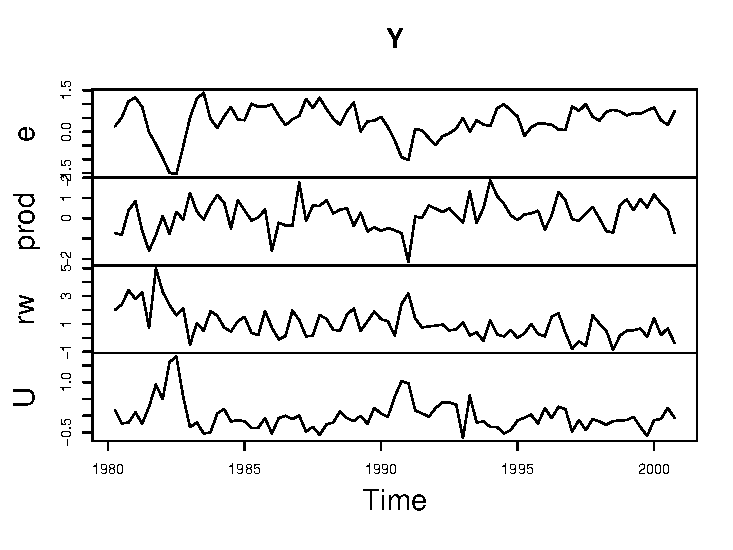
\includegraphics{article_jss_varshrink_files/figure-latex/diffCanada-1} 

}

\caption{\label{fig:diffCanada}The benchmark data set obtained by differencing the Canada data.}\label{fig:diffCanada}
\end{figure}
\end{CodeChunk}

The shrinkage methods are run with the option \code{const = "const"}
since the mean of the data has not been corrected. We set the lag order
\(p\) at \code{p} \(= 1, 2, 3\) to compare several VAR models. For the
semiparametric Bayesian method (\code{method = "sbayes"}), the degree of
freedom \(\nu\) was automatically selected. In addition, we ran the
K-fold CV method (\code{method = "kcv"}) for choosing \(\lambda\) and
\(\lambda_v\) values of the semiparametric Bayesian shrinkage estimator.

\begin{CodeChunk}

\begin{CodeInput}
R> set.seed(1000)
R> resu_model <- array(NA, dim = c(5, 2, 3),
R+   dimnames = list(c("Ridge regression", "Nonparametric shrinkage",
R+                     "Full Bayes", "Semi Bayes", "K-fold CV"),
R+                   c("AIC", "BIC"), c("p=1", "p=2", "p=3")))
R> for (p in 1:3) {
R+   EstimRidge <- VARshrink(Y, p = p, type = "const", method = "ridge")
R+   resu_model["Ridge regression", , p] <- c(AIC(EstimRidge), BIC(EstimRidge))
R+ 
R+   EstimNS <- VARshrink(Y, p = p, type = "const", method = "ns")
R+   resu_model["Nonparametric shrinkage", , p] <-
R+     c(AIC(EstimNS), BIC(EstimNS))
R+ 
R+   EstimFB <- VARshrink(Y, p = p, type = "const", method = "fbayes", dof = NULL)
R+   resu_model["Full Bayes", , p] <- c(AIC(EstimFB), BIC(EstimFB))
R+ 
R+   EstimSB <- VARshrink(Y, p = p, type = "const", method = "sbayes",
R+                        dof = NULL, prior_type = "NCJ")
R+   resu_model["Semi Bayes", , p] <- c(AIC(EstimSB), BIC(EstimSB))
R+ 
R+   EstimKCV <- VARshrink(Y, p = p, type = "const", method = "kcv",
R+                           dof = NULL, prior_type = "NCJ")
R+   resu_model["K-fold CV", , p] <- c(AIC(EstimKCV), BIC(EstimKCV))
R+ }
\end{CodeInput}
\end{CodeChunk}

We can compare several models by computing their AIC and BIC. The
following results in Table \ref{tab:modelcomp} indicate that the NS
method produced better VAR coefficients than those of the other methods,
and that the AIC took the minimum at \(p=3\) while the BIC took the
minimum at \(p=2\).

\begin{CodeChunk}
\begin{table}[t]

\caption{\label{tab:modelcomp}\label{tab:modelcomp}Information criteria (AIC, BIC) for model comparison.}
\centering
\begin{tabular}{l|r|r|r|r|r|r}
\hline
  & AIC.p=1 & BIC.p=1 & AIC.p=2 & BIC.p=2 & AIC.p=3 & BIC.p=3\\
\hline
Ridge regression & 465.8 & 504.6 & 442.9 & 509.3 & 445.3 & 525.9\\
\hline
Nonparametric shrinkage & 462.5 & 496.6 & 434.6 & 489.0 & 430.5 & 502.9\\
\hline
Full Bayes & 458.3 & 500.4 & 447.1 & 514.7 & 450.6 & 532.2\\
\hline
Semi Bayes & 502.6 & 549.6 & 483.8 & 567.3 & 496.2 & 607.8\\
\hline
K-fold CV & 526.9 & 574.3 & 477.2 & 526.2 & 469.6 & 540.0\\
\hline
\end{tabular}
\end{table}

\end{CodeChunk}

The estimated parameters by the NS method with \(p=2\) can be analyzed
further by using the methods and functions in Table \ref{tab:methods}.
For example, we can perform time series forecasting as in Figure
\ref{fig:pred}.

\begin{CodeChunk}

\begin{CodeInput}
R> plot(predict(VARshrink(Y, p = 2, type = "const", method = "ns")), names = "U")
\end{CodeInput}
\begin{figure}

{\centering 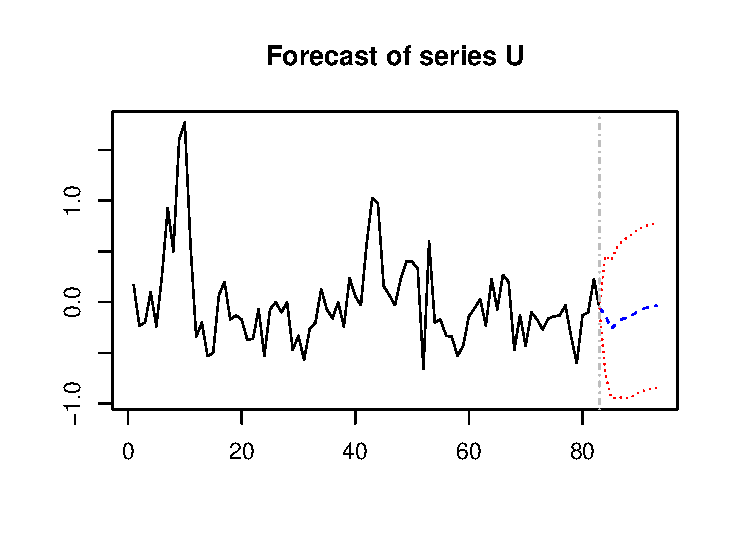
\includegraphics{article_jss_varshrink_files/figure-latex/pred-1} 

}

\caption{\label{fig:pred}A 10-step ahead Forecasting of time series by the VAR model estimated by the nonparametric shrinkage method. The differenced Canada data were modeled by a VAR(2) model selected at the minimum BIC.}\label{fig:pred}
\end{figure}
\end{CodeChunk}

\hypertarget{comparative-simulation}{%
\subsection{Comparative Simulation}\label{comparative-simulation}}

For comparison of estimation accuracies by the shrinkage estimation
methods, we generated multivariate time series data of length
\(T = 20, 40, 80, 160\) from \(K = 20\) dimensional VAR models of order
\(p = 1\). We note that when \(T = 20\), the sample size
\(N = T - p = 19\) becomes smaller than the dimensionality \(K = 20\).
We set the VAR coefficient matrix, \(\mathbf{A}_1\), to have the
diagonal entries of 0.6 and off-diagonal entries of zeros except for
\(K\) entries randomly selected on the lower triangular part of the
matrix. The nonzero off-diagonal entries were uniformly randomly drawn
from the interval \([-1, -0.2]\cup[0.2, 1]\). Since the coefficient
matrix is lower triangular, the diagonal entries determine its
eigenvalues, which lead to weak stationarity \citep{Hamilton94, Tsay05}.
The noise \(\boldsymbol\epsilon_t\) was randomly sampled from the
multivariate normal distribution whose covariance matrix has diagonal
entries of 1 and off-diagonal entries of 0.5. The mean of sum of squared
errors (MSSE) of estimated VAR coefficients, \(\widehat{\mathbf{A}}_1\),
was computed by \begin{equation}
    \sum_{i=1}^K \sum_{j=1}^K \left( \left(\widehat{\mathbf{A}}_1\right)_{ij} -
    \left(\mathbf{A}_1\right)_{ij}  \right)^2.
    \end{equation} We repeated the experiments 50 times and drew
boxplots to compare the SSEs of the shrinkage methods.

\begin{CodeChunk}

\begin{CodeInput}
R> set.seed(1000)
R> p <- 1; K <- 20; NumTimePTS <- c(20, 40, 80, 160)
R> const_vector <- c(rep(0.2, 5), rep(0.7, 15))
R> Sig <- diag(0.5, K) + matrix(0.5, K, K)
R> resu_SSE <- array(0, dim = c(50, 4, length(NumTimePTS)), dimnames =
R+   list(1:50, c("Ridge", "NS", "FBayes", "SBayes"), NumTimePTS))
R> for (idT in 1:length(NumTimePTS)) {
R+   numT = NumTimePTS[idT]
R+   for (r in 1:50) {
R+     Ad <- createVARCoefs_ltriangular(p = p, K = K, diag_val = 0.6,
R+             num_nonzero = K, const_vector = const_vector, range_max = 1)
R+     Md <- list(Coef = Ad, Sigma = Sig, dof = Inf)
R+     Y <- simVARmodel(numT = numT, model = Md, burnin = 20)
R+     EstimRG <- VARshrink(Y, p, "const", method = "ridge")
R+     EstimNS <- VARshrink(Y, p, "const", method = "ns")
R+     EstimFB <- VARshrink(Y, p, "const", method = "fbayes", dof = NULL)
R+     EstimSB <- VARshrink(Y, p, "const", method = "sbayes", prior_type = "NCJ")
R+     resu_SSE[r, 1, idT] <- calcSSE_Acoef(Acoef_sh(EstimRG), Ad$A)
R+     resu_SSE[r, 2, idT] <- calcSSE_Acoef(Acoef_sh(EstimNS), Ad$A)
R+     resu_SSE[r, 3, idT] <- calcSSE_Acoef(Acoef_sh(EstimFB), Ad$A)
R+     resu_SSE[r, 4, idT] <- calcSSE_Acoef(Acoef_sh(EstimSB), Ad$A)
R+   }
R+ }
\end{CodeInput}
\end{CodeChunk}

\begin{CodeChunk}
\begin{figure}

{\centering 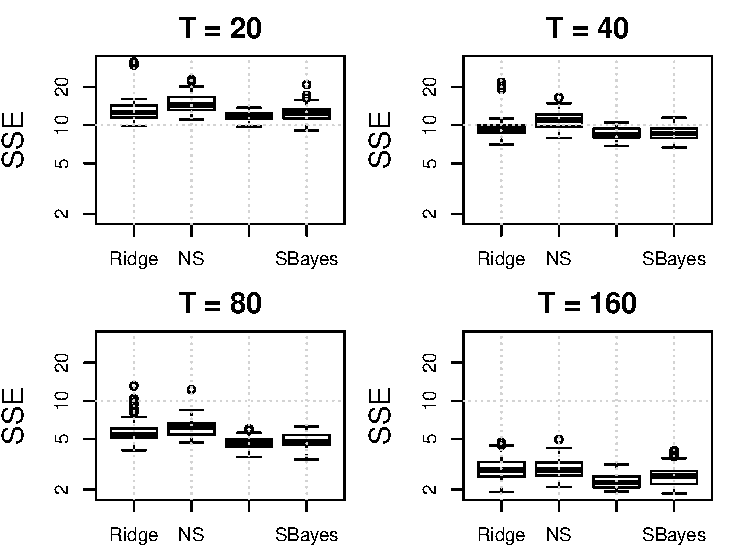
\includegraphics{article_jss_varshrink_files/figure-latex/comparisons_K20-1} 

}

\caption{\label{fig:comparisons_K20}Comparison of the mean of sum of squared errors (MSSE) of the VAR coefficients estimated by the four shrinkage methods. The multivariate time series data were randomly generated from VAR models of order $p = 1$ and dimensionality $K = 20$, and the noise term was randomly drawn from a multivariate normal distribution.}\label{fig:comparisons_K20}
\end{figure}
\end{CodeChunk}

\begin{CodeChunk}

\begin{CodeOutput}
pdf 
  2 
\end{CodeOutput}
\end{CodeChunk}

Figure \ref{fig:comparisons_K20} shows the boxplots of the MSSEs of the
VAR coefficients estimated by the four shrinkage methods. The full
Bayesian approach (FBayes) and the semiparametric Bayesian approach
(SBayes) yielded the best accuracies among the four methods.

\begin{center}\rule{0.5\linewidth}{\linethickness}\end{center}

\hypertarget{conclusions}{%
\section{Conclusions}\label{conclusions}}

We wrote an \proglang{R} software package \pkg{VARshrink} for shrinkage
estimation of VAR model parameters. The shrinkage methods included in
this package are the multivariate ridge regression
\citep{Hoerl70, Golub79}, a nonparametric shrinkage method
\citep{Rhein07c}, a full Bayesian shrinkage method \citep{Ni05}, and a
semiparametric Bayesian shrinkage method \citep{LeeChoiKim2016}. An
advantage of this package is the integration of the nonparametric,
parametric, and semiparametric methods in one frame via a common
interface function \code{VARshrink()}, which makes it easy and
convenient to use various types of shrinkage estimation methods.
Moreover, we note that the shrinkage estimation methods implemented in
the current version have not been widely implemented in \proglang{R}
packages in the context of VAR models.

We demonstrated the use of model selection criteria as AIC and BIC by
using benchmark time series data. We note that computation of the
log-likelihood of an estimated model must consider the actual
distribution assumption of each method. We explained that the
multivariate normal distribution is not the only choice for a
distribution of noise, but another distributions such as the
multivariate t-distribution can be chosen. Moreover, an effective number
of parameters must be calculated for computing the AIC and BIC values.
In this case, a large number of shrinkage parameter value leads to a
small value of the effective number of parameters. In the package
\pkg{VARshrink}, effective number of parameters is computed
automatically based on the selected shrinkage parameter value.

Shrinkage methods are quite crucial especially for high dimensional VAR
models. Bayesian approaches have been developed widely for VAR models in
the literature for various purposes. However, the computational time for
carrying out MCMC processes may be intractably high for high dimensional
VAR models. For this reason, it is important to use nonparametric and
semiparametric shrinkage estimation methods together to produce
computationally feasible estimates of model parameters. The \proglang{R}
package \pkg{VARshrink} is the first step to an integrative and general
types of software packages for VAR models. Moreover, this package can be
extended to include other shrinkage methods such as Bayesian shrinkage
methods using several types of different prior distributions.

\renewcommand\refname{References}
\bibliography{bibVARshrink.bib}


\end{document}

